% magick -quality 90 -density 1200 $input -resize 25% -trim $output

\documentclass{standalone}
\usepackage{tikz}

\usetikzlibrary{math,calc}


\begin{document}

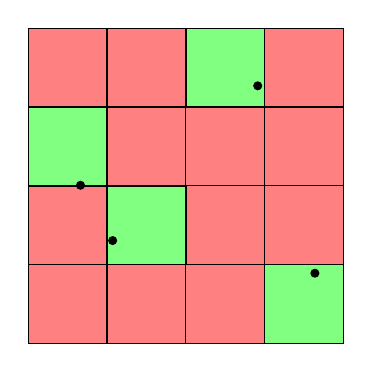
\begin{tikzpicture}
  \draw[fill=red!50] (0,0) rectangle (4,4);

  \foreach \i/\j in {1/3,2/2,3/4,4/1} {
    \tikzmath{
      real \x;
      real \y;
      \x = \i - random();
      \y = \j - random();
    }

    \draw[ultra thin,fill=green!50] (\i, \j) rectangle ++(-1, -1);

    \draw[fill=black] (\x, \y) circle [radius=0.05cm];
  }

  \draw (0,0) grid (4,4);
\end{tikzpicture}

\end{document}